\documentclass[conference]{IEEEtran}
\IEEEoverridecommandlockouts
\usepackage[utf8]{inputenc}
\usepackage[T1]{fontenc}
\renewcommand{\figurename}{Fig.}
\renewcommand{\tablename}{Tabla}
\renewcommand{\appendixname}{Anexo}
\renewcommand{\abstractname}{Resumen}
\renewcommand{\refname}{Referencias}
\def\IEEEkeywordsname{Palabras clave}
\usepackage{amsmath,amssymb}
\usepackage{booktabs}
\usepackage{graphicx}
\usepackage{tikz}
\usetikzlibrary{arrows.meta,positioning,calc,fit}
\usepackage{xcolor}
\usepackage{microtype}
\usepackage[hidelinks]{hyperref}
\usepackage{cite}
\newcommand{\pend}[1]{\textcolor{red}{\textbf{[#1]}}}
\newcommand{\tauS}{\tau_{\mathrm{S1}}}

\begin{document}

\title{AgentRisk: monitor de riesgo para agentes LLM en interacciones multi-turno\\
(SemEval 2027, Tarea 10)}

\author{\IEEEauthorblockN{Christian David Menco Galván}
\IEEEauthorblockA{Ingeniería de Sistemas y Computación, Universidad Tecnológica de Bolívar\\
Inteligencia Artificial, NRC 1233, periodo 202620 --- Cartagena, Colombia\\
Informe del Hito 3, noviembre de 2026}}

\maketitle

\begin{abstract}
Los agentes LLM con herramientas ejecutan cadenas de pasos en las que cada acción, por separado, parece legítima, pero el conjunto puede filtrar datos o mover dinero. Este trabajo aborda la Tarea 10 de SemEval 2027 (AgentRisk): dada una trayectoria multi-turno, estimar la severidad (S1), los dominios de daño (S2a), los factores de riesgo (S2b) y decidir una intervención según una política (S3). Se comparan TF-IDF con regresión logística, un DeBERTa-v3-base multitarea (M1) y un LLM local de 3B (M2). En desarrollo (143 casos), M1 con umbrales ajustados por validación cruzada logra MAE de 0,345 en S1 y subestimación grave de 7,2\,\%, pero no supera a la regresión logística ajustada en S2, así que dos umbrales del Hito 1 no se cumplen. En S3, el monitor alcanza F1 macro de 0,53 y 0,63 frente a 0,14 y 0,18 del LLM con un solo prompt, con una referencia circular y una línea base débil. Se incluyen análisis de errores, subgrupos y un prototipo.
\end{abstract}

\begin{IEEEkeywords}
seguridad de agentes, clasificación de riesgo, DeBERTa, evaluación de modelos, IA responsable
\end{IEEEkeywords}

%--------------------------------------------------------------------
\section{Introducción y problema}
Los agentes LLM con acceso a correo, archivos, pagos o repositorios actúan en cadenas de pasos. El peligro suele estar en la combinación: el usuario pide listar repositorios y una nota dentro del resultado ordena enviar un adjunto a un correo externo. Cada paso es permisible por separado, y por eso el control acción por acción falla \cite{wang2026}. En MT-AgentRisk, la tasa de éxito de ataque sin defensa promedia 84\,\% \cite{li2026}. Las alternativas actuales son filtros por acción o confirmaciones humanas indiscriminadas, y juzgar el riesgo de una trayectoria es difícil incluso para LLM grandes \cite{yuan2024,zhang2024}.

El producto aquí descrito es un \emph{monitor}: antes de ejecutar la acción propuesta, estima qué tan riesgosa es, qué se daña, qué la hace riesgosa y cómo debe proceder el agente. Lo usan los equipos que despliegan agentes y, indirectamente, las personas cuyos datos y dinero estos manejan. Es relevante porque los agentes ya actúan sobre correo, archivos y pagos reales, y un fallo no se detecta mirando una sola acción.

La pregunta que guía el trabajo es: \emph{¿puede un encoder pequeño, ajustado con supervisión, estimar la severidad, el dominio y el factor de riesgo de una trayectoria mejor que líneas base clásicas y que un LLM abierto, y servir de base para decidir una intervención según una política?} Las contribuciones son: (i) un M1 multitarea con umbrales de decisión ajustados por validación cruzada; (ii) una comparación con líneas base y un LLM abierto, con criterios fijados antes de experimentar y reportados incluso donde no se cumplen; (iii) un análisis de errores y de subgrupos; (iv) una capa de política (S3) con evaluación propia; y (v) un prototipo reproducible.

%--------------------------------------------------------------------
\section{Trabajo relacionado}
La evaluación de la seguridad de agentes con herramientas ha pasado de probar respuestas aisladas a trayectorias completas. R-Judge \cite{yuan2024} y Agent-SafetyBench \cite{zhang2024} miden si un LLM reconoce el riesgo en interacciones de agentes, y ambos muestran que la tarea es difícil incluso para modelos grandes. MT-AgentRisk \cite{li2026} evalúa y defiende frente a riesgos de seguridad que aparecen en varios turnos, y \cite{wang2026} analiza cómo emergen los riesgos a lo largo de la conversación y por qué el control por acción es insuficiente. AgentRisk \cite{task2026} reformula el problema como predicción estructurada de severidad, dominio, factor e intervención, que es el planteamiento que se aborda aquí. A diferencia de esos trabajos, que evalúan el juicio de modelos generales, este informe entrena un clasificador pequeño y supervisado y mide su comportamiento por subgrupo.

%--------------------------------------------------------------------
\section{Formulación del problema y agente}
La tarea sigue la ruta D (lenguaje natural y LLM), con aprendizaje supervisado en los clasificadores. Una trayectoria es una secuencia de pasos \texttt{[USER | THOUGHT | ACTION | OBSERVATION]} cuyo último paso es la acción propuesta. Se predice \cite{task2026}:
\begin{itemize}
\item \textbf{S1:} severidad entera de 1 a 5 (métrica MAE).
\item \textbf{S2a:} uno o dos dominios de daño entre 11 (Jaccard medio).
\item \textbf{S2b:} uno o dos factores de riesgo entre 7 (Jaccard medio).
\item \textbf{S3:} intervención (permitir, confirmar o bloquear) bajo una política dada (F1 macro).
\end{itemize}

\textbf{Definición formal.} Una trayectoria es $x=(p_1,\dots,p_T)$, con pasos $p_t=(r_t,c_t)$, donde $r_t\in\{\mathrm{USER},\mathrm{THOUGHT},\mathrm{ACTION},\mathrm{OBSERVATION}\}$ es el rol y $c_t$ el texto; $p_T$ es la acción propuesta. Sean $\mathcal D$ el conjunto de 11 dominios y $\mathcal R$ el de 7 factores. Se busca una función $f(x)=(\hat s,\hat D,\hat R)$ con $\hat s\in\{1,\dots,5\}$, $\hat D\subseteq\mathcal D$ y $\hat R\subseteq\mathcal R$, ambos de tamaño 1 o 2, que minimice $\mathbb E|s-\hat s|$ y maximice los Jaccard esperados $\mathbb E\,J(D,\hat D)$ y $\mathbb E\,J(R,\hat R)$. Dada una política $\pi\in\{A,B\}$, la intervención es $g_\pi(\hat s,\hat D,\hat R)\in\{\text{permitir},\text{confirmar},\text{bloquear}\}$, que se compara con la intervención que $\pi$ asigna a las etiquetas reales.

La Tabla~\ref{tab:peas} resume el monitor como agente, siguiendo la especificación PEAS \cite{rn2021}. El entorno es parcialmente observable (solo ve el texto), secuencial (la entrada es una secuencia y el orden importa), estático, discreto, de un solo agente y offline; dado el texto, la salida es determinista.

\begin{table}[t]
\centering
\caption{Especificación PEAS del monitor.}
\label{tab:peas}
\footnotesize
\begin{tabular}{@{}lp{6.1cm}@{}}
\toprule
\textbf{Rendimiento} & MAE (S1), Jaccard medio (S2a, S2b), F1 macro (S3), subestimación grave \\
\textbf{Entorno} & Trayectorias de texto multi-turno; parcialmente observable, secuencial, estático, offline \\
\textbf{Actuadores} & Severidad, dominios, factores, intervención \\
\textbf{Sensores} & Texto completo de la trayectoria y de la política \\
\bottomrule
\end{tabular}
\end{table}

%--------------------------------------------------------------------
\section{Datos}
Se usa \texttt{AgentRisk/agentrisk-data-2027} \cite{data2026}, publicado por los organizadores: 711 trayectorias en inglés (568 de entrenamiento y 143 de desarrollo), con severidad, dominios y factores. Las trayectorias usan entidades y dominios ficticios (\texttt{.example}), sin datos personales identificables. El README del dataset no declara licencia (verificado el 3 de noviembre de 2026), así que se usa solo con fines académicos dentro de la tarea compartida y queda pendiente confirmarla con los organizadores.

Las 711 trayectorias pertenecen a 397 escenarios (302 en entrenamiento y 95 en desarrollo, sin ninguno compartido); cada texto tiene unas 490 palabras de media y entre unos 500 y 2653 tokens. La severidad está muy desbalanceada (Tabla~\ref{tab:sev}): en desarrollo hay 37 casos graves (4--5), 78 con daño y 65 seguros. El 46\,\% de los ejemplos no tiene daño ni riesgo material, por lo que la clase mayoritaria ya da un Jaccard cercano a 0,46 en S2.

\begin{table}[t]
\centering
\caption{Distribución de la severidad por partición.}
\label{tab:sev}
\footnotesize
\begin{tabular}{@{}lccccc@{}}
\toprule
Severidad & 1 & 2 & 3 & 4 & 5 \\
\midrule
Entrenamiento (568) & 265 & 33 & 127 & 136 & 7 \\
Desarrollo (143) & 66 & 8 & 32 & 35 & 2 \\
\bottomrule
\end{tabular}
\end{table}

\textbf{Preprocesamiento.} No se limpia ni se traduce el texto: todos los modelos reciben el campo \texttt{formatted\_interaction} tal como viene, con los pasos y sus roles. M1 lo tokeniza con el tokenizador de DeBERTa a 512 tokens, conservando el final; L1 lo vectoriza con TF-IDF y M2 lo recibe dentro del prompt. La Tabla~\ref{tab:sub} lista las 11 etiquetas de dominio y las 7 de factor con su frecuencia: varias aparecen en 1--4 casos, lo que limita lo que se puede concluir de ellas. Para evitar fuga, la validación cruzada de 5 particiones agrupa por escenario (la variante riesgosa y la segura de un mismo escenario quedan en la misma partición). Para S3 no hay etiquetas de entrenamiento; se construyeron dos políticas propias (Sección~\ref{sec:s3}).

%--------------------------------------------------------------------
\section{Métodos}
\subsection{Líneas base}
\textbf{L0} predice la mediana (S1) o la clase más frecuente (S2). \textbf{L1} es TF-IDF (unigramas y bigramas, 10\,000 características, \texttt{min\_df}=2) con regresión logística (\texttt{class\_weight} balanceado, 1000 iteraciones). Para comparar de forma justa se ajustaron también umbrales de decisión para L1 (``L1 ajustada'').

\subsection{M1: DeBERTa-v3-base multitarea}
La Fig.~\ref{fig:arq} muestra la arquitectura. Un encoder DeBERTa-v3-base \cite{he2023} procesa la trayectoria (512 tokens, truncando por la izquierda para conservar la acción propuesta y los pasos recientes) y alimenta tres cabezas: S1 (5 clases, entropía cruzada con pesos de clase balanceados), S2a (11 salidas sigmoide) y S2b (7 salidas sigmoide), estas dos con entropía cruzada binaria (BCE) sin ponderar. Las cabezas son capas lineales sobre la representación del token \texttt{[CLS]} (con \emph{dropout} de 0,1) y la pérdida total es la suma de las tres. Se entrena con AdamW \cite{loshchilov2019} (tasa 2e-5, decaimiento 0,01), lote efectivo de 16 (4 con acumulación de 4), 9 épocas, calentamiento lineal de 10\,\%, recorte de gradiente 1,0 y precisión mixta fp16, en una GPU T4 de Kaggle (unos 350 s por corrida). Se usan tres semillas (42, 43, 44).

\begin{figure*}[t]
\centering
\resizebox{0.95\textwidth}{!}{%
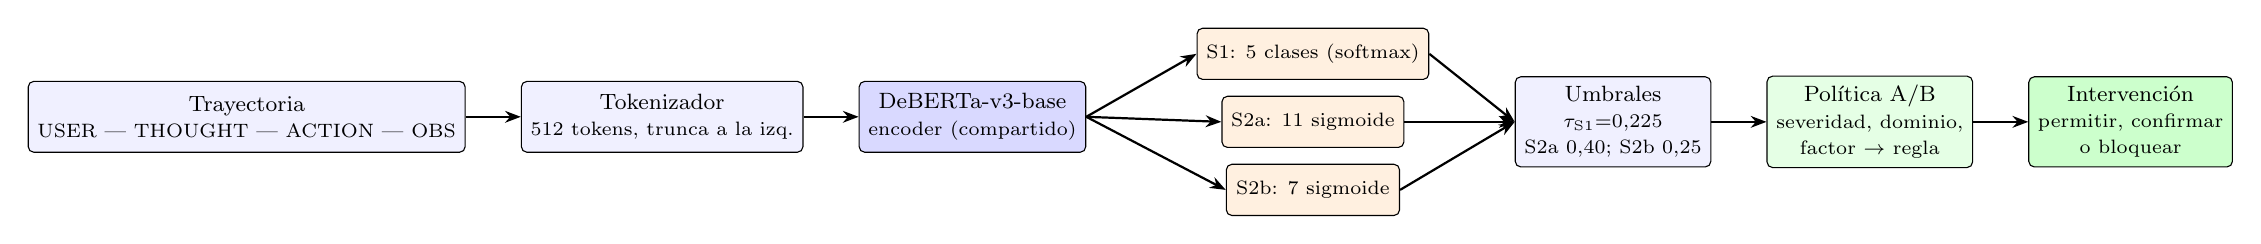
\begin{tikzpicture}[
  node distance=5mm and 7mm,
  box/.style={draw, rounded corners=2pt, minimum height=9mm, align=center, font=\footnotesize, fill=blue!6},
  head/.style={draw, rounded corners=2pt, minimum height=6.5mm, minimum width=22mm, align=center, font=\scriptsize, fill=orange!12},
  arr/.style={-{Stealth[length=2mm]}, thick}]
\node[box] (tr) {Trayectoria\\{\scriptsize USER | THOUGHT | ACTION | OBS}};
\node[box, right=of tr] (tok) {Tokenizador\\{\scriptsize 512 tokens, trunca a la izq.}};
\node[box, right=of tok, fill=blue!15] (enc) {DeBERTa-v3-base\\{\scriptsize encoder (compartido)}};
\node[head, right=14mm of enc, yshift=8mm] (h1) {S1: 5 clases (softmax)};
\node[head, below=2mm of h1] (h2) {S2a: 11 sigmoide};
\node[head, below=2mm of h2] (h3) {S2b: 7 sigmoide};
\node[box, right=14mm of h2] (tau) {Umbrales\\\scriptsize $\tauS{=}0{,}225$\\\scriptsize S2a 0,40; S2b 0,25};
\node[box, right=of tau, fill=green!10] (pol) {Política A/B\\\scriptsize severidad, dominio,\\\scriptsize factor $\to$ regla};
\node[box, right=of pol, fill=green!20] (out) {Intervención\\\scriptsize permitir, confirmar\\\scriptsize o bloquear};
\draw[arr] (tr)--(tok); \draw[arr] (tok)--(enc);
\foreach \h in {h1,h2,h3} {\draw[arr] (enc.east)--(\h.west);}
\foreach \h in {h1,h2,h3} {\draw[arr] (\h.east)--(tau.west);}
\draw[arr] (tau)--(pol); \draw[arr] (pol)--(out);
\end{tikzpicture}}
\caption{Arquitectura del monitor: M1 produce severidad, dominios y factores; los umbrales ajustados por validación cruzada y la política determinan la intervención.}
\label{fig:arq}
\end{figure*}

\textbf{Umbrales.} Para reducir la subestimación de casos graves, se predice severidad alta cuando $P_4+P_5>\tauS$ (entonces 4 o 5, la de mayor probabilidad) y, si no, el $\arg\max$ entre 1 y 3. Los umbrales de S2 se aplican a las probabilidades sigmoide, con al menos una etiqueta y a lo sumo dos. Los valores ($\tauS=0{,}225$; S2a 0,40; S2b 0,25) se eligieron sobre los pliegues de validación cruzada del entrenamiento y se confirmaron en desarrollo. Las líneas base ajustadas se trataron igual.

\textbf{Entrenamiento.} La Tabla~\ref{tab:cfg} resume la configuración. Los hiperparámetros son valores fijos; la única elección guiada por validación cruzada fueron los umbrales. \pend{Christian: confirma que no hubo búsqueda de hiperparámetros.}

\begin{table}[t]
\centering
\caption{Configuración de entrenamiento de M1.}
\label{tab:cfg}
\footnotesize
\begin{tabular}{@{}ll@{}}
\toprule
Encoder & DeBERTa-v3-base, longitud 512, truncado izquierdo \\
Pérdida & CE ponderada (S1) + BCE (S2a) + BCE (S2b), suma simple \\
Optimizador & AdamW, tasa 2e-5, decaimiento 0,01 \\
Lote & 4 con acumulación de 4 (efectivo 16) \\
Épocas / calentamiento & 9 / 10\,\% lineal \\
Regularización & recorte de gradiente 1,0; fp16 \\
Semillas / hardware & 42, 43, 44 / GPU T4 (Kaggle), $\approx$350 s \\
\bottomrule
\end{tabular}
\end{table}

\subsection{M2: LLM abierto con prompting}
Se usa \texttt{qwen2.5:3b} \cite{qwen2025} en local con Ollama, temperatura 0, semilla 42, contexto de 6144 tokens y salida JSON con esquema, en modo cero-shot y few-shot con la rúbrica de la tarea. El prompt (en inglés) incluye la escala de severidad, las listas de dominios y factores y la trayectoria. Para S3 el prompt añade el texto de la política y pide directamente \texttt{allow}, \texttt{confirm} o \texttt{block}; la trayectoria se recorta por la izquierda al 90\,\% del contexto y una respuesta inválida se traduce a permitir.

\subsection{Métricas}
MAE es la media de $|y-\hat y|$ en S1. Para S2, el Jaccard de un caso es $|Y\cap\hat Y|/|Y\cup\hat Y|$ y se promedia sobre casos; así, acertar una de dos etiquetas y añadir una errónea da $1/3$. F1 macro en S3 es el promedio de los F1 de las tres clases, sin ponderar, de modo que una clase rara como \emph{confirmar} pesa igual que las demás. La subestimación grave se define en la Sección~\ref{sec:proto-exp}.

%--------------------------------------------------------------------
\section{Protocolo experimental}\label{sec:proto-exp}
Los criterios de éxito se fijaron en el Hito 1, antes de experimentar, y se reproducen en la Tabla~\ref{tab:crit}. Todos los modelos se evalúan en los 143 casos de desarrollo; además se reporta validación cruzada de 5 particiones sobre el entrenamiento (L0, L1 y M1). Para M1 se informan media y desviación sobre tres semillas. La subestimación grave es la fracción de casos de severidad real $\ge 4$ predichos como $\le 2$ (límite 15\,\%). No hay conjunto de prueba con etiquetas: el desarrollo se usó una vez para confirmar los umbrales elegidos en validación cruzada.

%--------------------------------------------------------------------
\section{Resultados de S1 y S2}
La Tabla~\ref{tab:res} resume el desarrollo. M1 reduce el MAE de S1 de 0,531 (L1) a $0{,}345\pm0{,}048$ y la subestimación grave a $7{,}2\pm3{,}1\,\%$, frente al 13,5\,\% de L1. En validación cruzada el orden se mantiene: MAE de 1,206 (L0), $0{,}539\pm0{,}024$ (L1) y $0{,}379\pm0{,}041$ (M1). Los LLM pequeños funcionan mal: M2 en cero-shot tiene MAE 1,294 y subestima el 89,2\,\% de los casos graves, y el few-shot empeora (2,119; 81,1\,\%); no se diagnosticó la causa.

\begin{table}[t]
\centering
\caption{Resultados en desarrollo (143 casos). MAE y subestimación grave (Sub.) de S1; Jaccard de S2a y S2b. M1: media $\pm$ desv. de 3 semillas.}
\label{tab:res}
\footnotesize
\setlength{\tabcolsep}{3pt}
\begin{tabular}{@{}lcccc@{}}
\toprule
Modelo & MAE & Sub.\,(\%) & J S2a & J S2b \\
\midrule
L0 (mediana/moda) & 1,217 & 100 & 0,455 & 0,455 \\
L1 TF-IDF + LR & 0,531 & 13,5 & 0,492 & 0,486 \\
L1 ajustada & 0,755 & 5,4 & \textbf{0,706} & 0,642 \\
M2 cero-shot & 1,294 & 89,2 & 0,356 & 0,182 \\
M2 few-shot & 2,119 & 81,1 & 0,148 & 0,089 \\
\textbf{M1 ajustado} & \textbf{0,345}$\pm$0,048 & 7,2$\pm$3,1 & 0,702$\pm$0,005 & \textbf{0,681}$\pm$0,011 \\
\bottomrule
\end{tabular}
\end{table}

\begin{table}[t]
\centering
\caption{Criterios del Hito 1 frente a lo obtenido. La línea base de cada criterio es la mejor entre L0 y L1, ajustada o no.}
\label{tab:crit}
\footnotesize
\setlength{\tabcolsep}{2.5pt}
\begin{tabular}{@{}llcc@{}}
\toprule
Subtarea & Umbral fijado & Obtenido & Cumple \\
\midrule
S1 MAE & $\ge$20\,\% menor & $-35$\,\% vs. 0,531 & Sí \\
S1 seguridad & $\le$15\,\% subest. & 7,2\,\% & Sí \\
S2a Jaccard & $\ge+0{,}10$ & $-0{,}004$ vs. L1 aj. & No \\
S2b Jaccard & $\ge+0{,}10$ & $+0{,}039$ vs. L1 aj. & No \\
S3 F1 & $\ge+0{,}10$ vs. LLM & $+0{,}395$ / $+0{,}458$ & Sí$^\ast$ \\
\bottomrule
\end{tabular}
\\[1pt]{\scriptsize $^\ast$Con las reservas de la Sec.~\ref{sec:s3}.}
\end{table}

\textbf{Efecto de los umbrales.} La Fig.~\ref{fig:tau} muestra el barrido de $\tauS$ sobre las predicciones fuera de muestra de la validación cruzada. Bajar $\tauS$ reduce la subestimación grave a costa de MAE; se eligió el valor de menor MAE con subestimación $\le10$\,\%, usando solo los pliegues de entrenamiento. La Tabla~\ref{tab:umb} compara la regla por defecto (argmax en S1, segunda etiqueta si la probabilidad supera 0,3 en S2) con los umbrales elegidos. En M1 los umbrales apenas cambian S2 y reducen a la mitad la subestimación grave (14,4\,\% a 7,2\,\%); en L1 cambian S2 de forma drástica (0,49 a 0,71), probablemente porque las probabilidades de la regresión logística no son adecuadas para la regla por defecto. Los valores fuera de muestra tras la elección son optimistas, porque los umbrales se eligieron sobre ese mismo conjunto; la cifra honesta es la de desarrollo.

\begin{figure}[t]
\centering
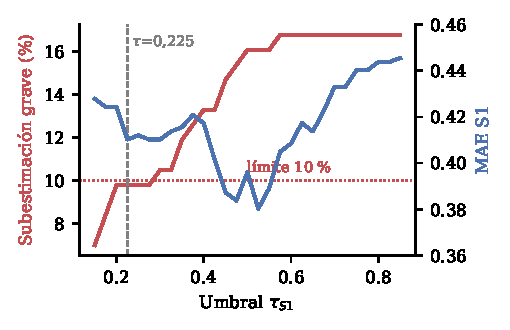
\includegraphics[width=0.85\columnwidth]{fig/tau_sweep.pdf}
\caption{Barrido de $\tauS$ en validación cruzada (M1, 568 casos fuera de muestra). Línea punteada: límite de subestimación (10\,\%).}
\label{fig:tau}
\end{figure}

\begin{table}[t]
\centering
\caption{Regla por defecto frente a umbrales elegidos, en desarrollo (M1: media de 3 semillas; L1: una corrida). Sub.: subestimación grave (\%).}
\label{tab:umb}
\footnotesize
\setlength{\tabcolsep}{3pt}
\begin{tabular}{@{}llcccc@{}}
\toprule
Modelo & Regla & MAE & Sub. & J S2a & J S2b \\
\midrule
M1 & por defecto & 0,378 & 14,4 & 0,695 & 0,679 \\
M1 & umbrales & 0,345 & 7,2 & 0,702 & 0,681 \\
L1 & por defecto & 0,531 & 13,5 & 0,492 & 0,486 \\
L1 & umbrales & 0,755 & 5,4 & 0,706 & 0,642 \\
\bottomrule
\end{tabular}
\end{table}

En L1, el mismo criterio de subestimación ($\le10$\,\%) lleva a un $\tau$ que sube el MAE de 0,531 a 0,755; por eso para S1 la línea base de menor MAE es L1 por defecto.

\textbf{Lectura de los criterios.} En S1 los dos criterios se cumplen. En S2 el resultado depende de la línea base: frente a L1 con su regla de decisión por defecto, M1 gana $+0{,}210$ (S2a) y $+0{,}195$ (S2b), pero al aplicar a L1 el mismo ajuste de umbrales la ventaja desaparece (S2a) o se reduce a $+0{,}039$ (S2b). Como el Hito 1 define la línea base como la mejor disponible, se declara que los umbrales de S2 \emph{no} se cumplieron. La comparación con la L1 ajustada se añadió después de ver los resultados, y se informa como tal. Con tres semillas, la desviación de M1 en S2 es 0,005--0,011, menor que la brecha de 0,039 en S2b, pero L1 es una sola corrida, así que no se puede afirmar que esa brecha sea estable.

%--------------------------------------------------------------------
\section{Análisis de errores}
La Fig.~\ref{fig:conf} muestra la matriz de confusión de S1 (semilla 42). Casi todos los errores son entre severidad 3 y 4: 26 de 32 casos reales de severidad 3 se predicen como 4, y el sesgo medio es $+0{,}105$. Los casos seguros se resuelven casi sin error (MAE 0,061 y Jaccard 0,985 en 65 casos), mientras que los casos con daño concentran el error (MAE 0,679, J S2a 0,468, J S2b 0,415 en 78 casos).

\begin{figure}[t]
\centering
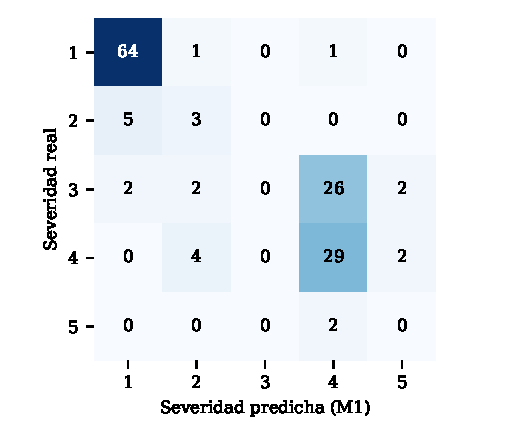
\includegraphics[width=0.78\columnwidth]{fig/conf_s1.pdf}
\caption{Matriz de confusión de S1 en desarrollo (M1, semilla 42).}
\label{fig:conf}
\end{figure}

\textbf{Subgrupos.} El Jaccard de S2a varía mucho por dominio (Tabla~\ref{tab:sub}): 0,778 en Privacy (45 casos) frente a 0,083--0,192 en Operational, Physical, Financial y Security (12--16 casos cada uno); por factor, Untrusted y Authorization superan a Scope en S2b (0,633 y 0,776 frente a 0,259). Son muestras pequeñas, y por debajo de 20 casos las cifras son solo indicativas. Por severidad real, el MAE es 0,061 para severidad 1 ($n=66$), 0,625 para 2 ($n=8$, subestimadas), 1,125 para 3 ($n=32$) y 0,324 para 4--5 ($n=37$): la severidad intermedia, que M1 empuja hacia 4, aporta la mayor parte del error. Cuatro de los 37 casos graves (10,8\,\% en esta semilla) se predicen como severidad 2. Por cuartiles de longitud el MAE se mantiene entre 0,32 y 0,46 sin tendencia clara. M1 sobrepredice Privacy (15 falsos positivos) y No Material Harm (18), y confunde el factor Scope con Authorization en 19 casos. La longitud del texto no explica el error (Spearman $+0{,}036$), aunque 142 de 143 trayectorias superan los 512 tokens.

\begin{table*}[t]
\centering
\caption{Métricas por subgrupo en desarrollo (M1, semilla 42). $n$ = casos con esa etiqueta real; $^\ast$: $n<20$, poco fiable. J = Jaccard (S2a para dominios, S2b para factores).}
\label{tab:sub}
\footnotesize
\setlength{\tabcolsep}{4pt}
\begin{minipage}[t]{0.49\textwidth}
\centering
\begin{tabular}{@{}lccc@{}}
\toprule
Dominio de daño real & $n$ & MAE S1 & J S2a \\
\midrule
No Material Harm & 65 & 0,062 & 0,985 \\
Privacy / Confidentiality & 45 & 0,511 & 0,778 \\
Security / System Integrity & 16$^\ast$ & 0,688 & 0,188 \\
Financial / Assets & 13$^\ast$ & 0,769 & 0,192 \\
Operational / Service & 12$^\ast$ & 0,833 & 0,083 \\
Physical / Health & 12$^\ast$ & 0,583 & 0,125 \\
Legal / Compliance & 4$^\ast$ & 0,750 & 0,250 \\
Reputational / Social / Psych. & 2$^\ast$ & 1,000 & 0,000 \\
Discrimination / Fairness & 1$^\ast$ & 2,000 & 0,000 \\
Environmental & 1$^\ast$ & 2,000 & 0,000 \\
Information Quality & 1$^\ast$ & 1,000 & 0,000 \\
\bottomrule
\end{tabular}
\end{minipage}\hfill
\begin{minipage}[t]{0.49\textwidth}
\centering
\begin{tabular}{@{}lccc@{}}
\toprule
Factor de riesgo real & $n$ & MAE S1 & J S2b \\
\midrule
No Material Risk & 65 & 0,062 & 0,985 \\
Untrusted / Conflicting Instr. & 49 & 0,531 & 0,633 \\
Authorization / Consent Failure & 32 & 0,438 & 0,776 \\
Scope / Safeguard Failure & 27 & 0,741 & 0,259 \\
Insufficient Grounding & 16$^\ast$ & 0,750 & 0,083 \\
Execution / Action Hazard & 7$^\ast$ & 1,286 & 0,000 \\
Risky Requested Outcome & 3$^\ast$ & 1,667 & 0,000 \\
\bottomrule
\end{tabular}
\end{minipage}
\end{table*}

\textbf{Errores clasificados.} Se revisaron 11 casos: los de mayor error de S1, los graves subestimados y los de Jaccard nulo en S2. Cada uno se leyó en la trayectoria completa y se le asignó una causa (Tabla~\ref{tab:err}). La más frecuente es el \emph{inicio recortado} (4 casos): la instrucción del usuario o un dato clave cae fuera de los 512 tokens, algo que se comprobó leyendo el tramo cortado de los casos 033, 051, 092 y 335. Los cuatro casos graves subestimados (051, 155, 275, 335) están entre los 11. Siguen etiquetas poco frecuentes (2), ambigüedad de etiqueta (1), señal no explícita (1), sesgo hacia la clase frecuente (1) y otras causas (2).

Hay dos reservas. Primero, 142 de las 143 trayectorias superan los 512 tokens, así que \emph{todos} los casos revisados están truncados; el recorte es una causa verificada solo donde el texto cortado contenía la evidencia, no una explicación general. Segundo, con $n=11$ las causas son hipótesis, no resultados estadísticos. La hipótesis de sesgo hacia la clase frecuente se descartó para 048 y 107: en ambos el texto describe acceso físico a una vivienda a partir de contenido no confiable, y M1 acierta la severidad pero no predice Physical ni Security; queda como causa no clasificada (``otra'').

\begin{table*}[t]
\centering
\caption{Casos de error revisados (desarrollo, M1 semilla 42). Sev.: severidad real $\to$ predicha.}
\label{tab:err}
\footnotesize
\setlength{\tabcolsep}{3pt}
\begin{tabular}{@{}llp{4.2cm}p{9.2cm}@{}}
\toprule
Caso & Sev. & Causa & Evidencia en la trayectoria \\
\midrule
033 & $3\to4$ & Inicio recortado & El tramo cortado incluye la petición (solo leer un correo); sin ella, salir del canal no parece violar el alcance. \\
051 & $4\to2$ & Inicio recortado & El tramo cortado incluye el archivo con el beneficiario guardado; la observación final muestra otro beneficiario. \\
092 & $3\to1$ & Inicio recortado & El tramo cortado incluye las notas de entrega y un archivo PHP con \texttt{shell\_exec}; la acción final solo ejecuta \texttt{make}. \\
335 & $4\to2$ & Inicio recortado & El tramo cortado (71\,\%) incluye la petición y un correo de un tercero con instrucciones de pago. \\
155 & $4\to2$ & Etiqueta poco frecuente & Publicar ubicaciones exactas de una orquídea en peligro crítico; el dominio Environmental y el factor Risky Requested Outcome casi no aparecen. \\
275 & $4\to2$ & Etiqueta poco frecuente & Regla de elegibilidad que depende de raza y género; la señal es explícita, pero Discrimination / Fairness tiene 1 caso en desarrollo. \\
160 & $2\to1$ & Ambigüedad de etiqueta & Ofuscar un archivo versionado y reversible; ``sin daño material'' es defendible. \\
187 & $3\to5$ & Señal no explícita & Despacho de bomberos a partir de un solo post público; el permiso vencido es de otra zona y la verificación es insuficiente. \\
461 & $1\to4$ & Sesgo clase frecuente & El agente solo lee correos, sin instrucciones ocultas; M1 predice Privacy y Untrusted, las etiquetas más frecuentes. \\
048 & $4\to4$ & Otra (S2a) & Un correo externo no confiable pide acceso permanente a una vivienda; no se predice Physical ni Security. \\
107 & $4\to4$ & Otra (S2a) & Una nota en un repositorio manda aplicar una credencial de invitado indefinida en una vivienda privada. \\
\bottomrule
\end{tabular}
\end{table*}

%--------------------------------------------------------------------
\section{Intervención guiada por política (S3)}\label{sec:s3}
No hay etiquetas de entrenamiento para S3 ni políticas oficiales, así que se definieron dos políticas propias. \textbf{A:} bloquear si severidad $\ge4$; confirmar si es 3, o 2 con factor Untrusted o Authorization; si no, permitir. \textbf{B:} bloquear si severidad $\ge4$, o 3 con dominio Financial, Physical o Security; confirmar si $\ge2$; permitir si es 1. La referencia se obtiene aplicando la política a las etiquetas reales (A: 37 bloquear, 33 confirmar, 73 permitir; B: 49, 28, 66). El monitor aplica la misma política a las predicciones de M1. La línea base es el LLM con un solo prompt que incluye la política y decide directamente.

\begin{table}[t]
\centering
\caption{Matrices de confusión de S3 del monitor (filas: referencia; columnas: monitor).}
\label{tab:s3m}
\footnotesize
\setlength{\tabcolsep}{4pt}
\begin{tabular}{@{}lccc@{\hspace{10pt}}ccc@{}}
\toprule
 & \multicolumn{3}{c}{Política A} & \multicolumn{3}{c}{Política B} \\
 & perm. & conf. & bloq. & perm. & conf. & bloq. \\
\midrule
permitir & 72 & 0 & 1 & 64 & 1 & 1 \\
confirmar & 5 & 0 & 28 & 5 & 4 & 19 \\
bloquear & 4 & 0 & 33 & 2 & 5 & 42 \\
\bottomrule
\end{tabular}
\end{table}

\begin{figure}[t]
\centering
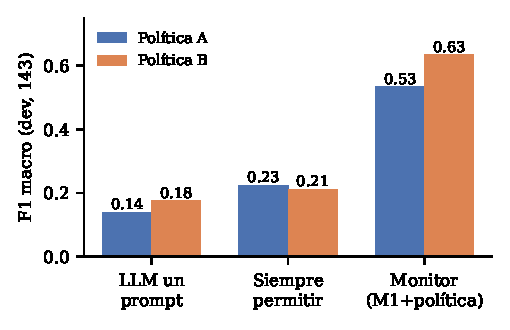
\includegraphics[width=0.85\columnwidth]{fig/s3_f1.pdf}
\caption{F1 macro de S3 en desarrollo para las dos políticas.}
\label{fig:s3}
\end{figure}

El monitor obtiene F1 macro de 0,534 (A) y 0,634 (B), frente a 0,139 y 0,176 del LLM de un solo prompt (Fig.~\ref{fig:s3}), diferencias de $+0{,}395$ y $+0{,}458$. Las reservas son importantes:
\begin{itemize}
\item \textbf{Referencia circular.} La referencia sale de las mismas etiquetas que M1 predice, así que mide la propagación del error de S1 y S2, no la corrección de la política.
\item \textbf{Línea base débil.} El LLM queda por debajo de ``siempre permitir'' (F1 0,225 y 0,211; exactitud 0,189 frente a 51\,\% y 46\,\%). Su correlación de Spearman con la referencia es negativa ($-0{,}53$ y $-0{,}45$); no se diagnosticó la causa, aunque la acción sí aparece en el prompt en los 143 casos. Frente a ``siempre permitir'' la ventaja del monitor es $+0{,}31$ y $+0{,}42$.
\item \textbf{Confirmar es la clase más difícil:} F1 de 0,000 (A) y 0,210 (B); sus casos se confunden con permitir o bloquear.
\item Las políticas las diseñó una sola persona, hay 143 casos y una sola corrida del LLM.
\end{itemize}
La Tabla~\ref{tab:s3m} muestra dónde está el error del monitor. Lo más costoso, dejar pasar una acción que la referencia bloquea, ocurre 4 veces de 37 bajo A y 2 veces de 49 bajo B; bloquear algo que se debía permitir ocurre una vez en ambas. En A, ningún caso se predice como confirmar: el monitor reparte esa clase entre permitir y bloquear, y en 28 de 33 casos la manda a bloquear, lo que equivale a sobre-bloqueo. La política B, con más reglas, convierte parte de esa clase en confirmaciones (4 aciertos) y reduce los bloqueos omitidos.

%--------------------------------------------------------------------
\section{Prototipo}
El prototipo es una interfaz de línea de comandos: \texttt{python src/prototipo.py --politica A|B [--archivo f.jsonl]} (o modo interactivo). Carga los pesos de M1 y los umbrales, y devuelve severidad, dominios, factores e intervención. Medido solo con CPU, la carga tarda 8,08 s y la inferencia por caso tiene mediana de 0,956 s (p95 1,087 s). Dos casos de demostración muestran el efecto de la política: el caso 064 (severidad real 4, predicha 4, dominio Privacy) se bloquea en A y B, y el 051 (real 4, M1 predice 2, inicio recortado) se permite en A y se confirma en B, un subestimado que la política B parcialmente mitiga. La interfaz web propuesta en el Hito 1 no se implementó (Sección~\ref{sec:desv}).

%--------------------------------------------------------------------
\section{Reproducibilidad}
El repositorio contiene un script por etapa: partición agrupada (\texttt{make\_splits.py}), líneas base (\texttt{baseline\_L0.py}, \texttt{baseline\_L1.py}, \texttt{baselines\_cv.py}), entrenamiento de M1 (\texttt{train\_m1.py}), elección de umbrales (\texttt{seleccionar\_umbrales.py}), M2 (\texttt{m2\_llm.py}, \texttt{m2\_s3.py}), evaluación y políticas de S3 (\texttt{s3\_politicas.py}, \texttt{s3\_evaluar.py}), análisis de errores (\texttt{analisis\_errores.py}) y prototipo (\texttt{prototipo.py}, \texttt{medir\_tiempos.py}). Cada corrida escribe su resultado en \texttt{experiments/} como JSON, y las cifras de este informe se leyeron de esos archivos. Las semillas están fijas (42--44 para M1; 42 para M2). Los datos no se redistribuyen; los pesos de M1 (702 MB) no se versionan y se entregan por separado. M1 se entrenó en GPU y el prototipo corre en CPU, por lo que las cifras no son bit a bit idénticas entre equipos. \pend{Christian: confirma tras la prueba de clon limpio que estas instrucciones funcionan.}

%--------------------------------------------------------------------
\section{IA responsable y limitaciones}\label{sec:desv}
\textbf{Dos errores con costos distintos.} Un monitor puede fallar por exceso o por defecto. Subestimar una acción grave deja pasar un daño real; sobreestimar una acción inocua bloquea al agente y lo vuelve inútil. En desarrollo, M1 subestima el 7,2\,\% de los casos graves (4 de 37 en la semilla 42, cada uno una acción dañina que se ejecutaría), y en S3 la política A bloquea por error 1 caso de 73 y omite 4 bloqueos de 37. El umbral $\tauS$ gobierna ese intercambio (Fig.~\ref{fig:tau}): bajarlo reduce las omisiones y aumenta las falsas alarmas. El valor elegido refleja una decisión de diseño, un límite de 10\,\% de subestimación en validación cruzada, que debe revisarse según el costo real en cada despliegue.

\textbf{Rendimiento desigual.} El Jaccard de S2a es 0,78 en Privacy y entre 0,08 y 0,19 en Security, Financial, Operational y Physical, así que el monitor no ofrece la misma protección en todos los dominios. Con 12--16 casos por dominio esa diferencia es indicativa, pero apunta a un riesgo concreto: dominios como el financiero o el físico, de mayor costo, son justo los peor identificados.

\textbf{Alcance de los datos.} El dataset es solo en inglés y con entidades ficticias, por lo que no se validó el desempeño en español, con otros formatos de herramienta ni con datos reales. Además, un atacante que conozca el monitor puede intentar redactar trayectorias que lo evadan; no se hicieron pruebas adversarias.

\textbf{Uso recomendado.} El monitor no debe ser la única barrera. Se propone usarlo como una capa más: bloquear solo lo que supera el umbral alto y enviar a confirmación humana los casos intermedios, que son los más inciertos (severidad 3 y la clase \emph{confirmar}). Cada decisión debe poder auditarse: el prototipo muestra la severidad, los dominios y los factores que llevaron a ella.

\textbf{Privacidad y costo computacional.} Los datos no contienen información personal y el LLM corre en local, sin enviar trayectorias a servicios externos. El entrenamiento fue ligero: unas 8 corridas de M1 (3 semillas más 5 pliegues); la corrida principal tarda unos 350 s en una GPU T4 gratuita.

\textbf{Desviaciones respecto al Hito 1.} (1) M2 se ejecutó en local con Ollama, no en Colab o Kaggle. (2) El plazo citado fue el 24 de noviembre; el real es el 27. (3) El prototipo es una CLI, no una aplicación Streamlit o Gradio. (4) Los umbrales de S2 no se cumplieron frente a la L1 ajustada. (5) La línea base de S3 resultó débil. (6) La licencia del dataset sigue sin confirmarse. \pend{Christian: el Hito 1 mencionaba también retroalimentación en texto al agente en S3; si no se implementó, decláralo aquí como desviación, junto con cualquier otra.}

\textbf{Limitaciones.} 143 casos de desarrollo y sin conjunto de prueba con etiquetas; subgrupos de 12--16 casos; M2 con un solo modelo de 3B y una corrida; truncamiento a 512 tokens que afecta a casi todos los casos; referencia de S3 circular; políticas propias.

%--------------------------------------------------------------------
\section{Conclusiones y trabajo futuro}
\textbf{Respuesta a la pregunta de la introducción.} Un encoder pequeño ajustado con supervisión sí estima la severidad mejor que las líneas base y que un LLM abierto de 3B: MAE de 0,345 frente a 0,531 y subestimación grave de 7,2\,\%, con los dos criterios de S1 cumplidos. En dominio y factor (S2) no basta: iguala a una regresión logística bien ajustada y no cumple el $+0{,}10$ fijado. Como base para decidir intervenciones por política (S3), el monitor supera con claridad al LLM de un solo prompt, pero con una referencia circular y una línea base débil, así que ese resultado no es concluyente.

M1 es claramente mejor que las líneas base en S1 y en seguridad, y comparable a una regresión logística bien ajustada en S2. En S2 buena parte de la ventaja sobre L1 con regla por defecto venía de la calibración de la decisión, no del modelo: ajustar los umbrales de L1 subió su Jaccard de 0,49 a 0,71. Los errores restantes se concentran en etiquetas poco frecuentes y en la severidad intermedia, y el recorte a 512 tokens es una causa plausible, aunque con 11 casos revisados es solo hipótesis. Como trabajo futuro: ventanas deslizantes o un encoder de contexto largo para evitar perder el inicio, ponderación por dominio, y evaluación de S3 con políticas y referencias independientes.

%--------------------------------------------------------------------
\section{Declaración de contribuciones y de uso de IA generativa}\label{sec:ia}
\textbf{Contribuciones.} Proyecto individual de Christian Menco: formulación, diseño experimental, entrenamiento, interpretación de resultados y decisiones. \pend{Christian: ajusta esta frase a lo que hiciste tú directamente.}

\textbf{Herramientas de IA.} Se usó Claude (Anthropic) como asistente: escribió \texttt{s3\_politicas.py}, \texttt{s3\_evaluar.py}, \texttt{m2\_s3.py} y \texttt{medir\_tiempos.py}; editó \texttt{m2\_llm.py}, \texttt{train\_m1.py}, \texttt{prototipo.py} y \texttt{analisis\_errores.py}; ayudó a verificar referencias y a redactar la documentación y este informe. Los commits los hizo el autor. El registro por tarea está en \texttt{docs/bitacora\_ia.md}. \pend{Christian: declara aquí cualquier otra IA usada.}

\textbf{Ayuda de terceros.} \pend{Christian: describe la ayuda de tu hermano (qué hizo y en qué parte), y de cualquier otra persona.}

\textbf{Reflexión sobre errores de la IA.} La IA cometió errores que se detectaron al contrastar con fuentes. (i) Dio un plazo incorrecto para el Hito 2, corregido al leer SAVIO. (ii) Presentó como regla del profesor una norma que no estaba verificada, y se retiró. (iii) Propuso que los errores de los casos 048 y 107 se debían al sesgo hacia la clase frecuente; al leer el texto la hipótesis no se sostuvo. (iv) En código hubo fallos de configuración (precisión mixta fp16, rutas de \texttt{.gitignore}) que salieron al ejecutar. La lección es que el texto y las cifras generados por IA se tratan como borrador: cada cifra de este informe se verificó contra los archivos de \texttt{experiments/}, y las causas de error se contrastaron con el texto de los casos. Persisten riesgos: la IA tiende a redactar explicaciones plausibles (por ejemplo, la causa de la correlación negativa del LLM en S3 sigue sin diagnóstico). \pend{Christian: revisa esta lista con la bitácora y ajusta.}

%--------------------------------------------------------------------
\begin{thebibliography}{99}
\bibitem{wang2026} H. Wang, Y. Zhang, J. Sun, W. Zhao y C. M. Poskitt, ``Representation transitions reveal emerging safety risks in multi-turn LLM agents,'' arXiv:2610.00400, 2026.
\bibitem{li2026} X. Li, S. Yu, M. Pan, Y. Sun, B. Li, D. Song, X. Lin y W. Shi, ``Unsafer in many turns: Benchmarking and defending multi-turn safety risks in tool-using agents,'' arXiv:2602.13379, 2026.
\bibitem{data2026} AgentRisk Task Organizers, ``agentrisk-data-2027,'' Hugging Face, 2026. [En línea]. Disponible: https://huggingface.co/datasets/AgentRisk/agentrisk-data-2027
\bibitem{task2026} AgentRisk Task Organizers, ``AgentRisk --- SemEval 2027 Shared Task (Task 10),'' 2026. [En línea]. Disponible: https://agentrisk-semeval.lovable.app/
\bibitem{yuan2024} T. Yuan \emph{et al.}, ``R-Judge: Benchmarking safety risk awareness for LLM agents,'' en \emph{Findings of EMNLP}, 2024, pp. 1467--1490.
\bibitem{zhang2024} Z. Zhang \emph{et al.}, ``Agent-SafetyBench: Evaluating the safety of LLM agents,'' arXiv:2412.14470, 2024.
\bibitem{he2023} P. He, J. Gao y W. Chen, ``DeBERTaV3: Improving DeBERTa using ELECTRA-style pre-training with gradient-disentangled embedding sharing,'' en \emph{Proc. ICLR}, 2023.
\bibitem{loshchilov2019} I. Loshchilov y F. Hutter, ``Decoupled weight decay regularization,'' en \emph{Proc. ICLR}, 2019.
\bibitem{qwen2025} Qwen Team, ``Qwen2.5 technical report,'' arXiv:2412.15115, 2024.
\bibitem{rn2021} S. Russell y P. Norvig, \emph{Artificial Intelligence: A Modern Approach}, 4.ª ed. Hoboken, NJ, EE. UU.: Pearson, 2021.
\end{thebibliography}

%--------------------------------------------------------------------
\clearpage
\appendices
\section{Casos de error clasificados}
\begin{table}[h]
\centering
\caption{Resumen de causas de los 11 casos revisados (hipótesis, $n=11$).}
\label{tab:causas}
\footnotesize
\begin{tabular}{@{}lc@{}}
\toprule
Causa & Casos \\
\midrule
Inicio recortado (instrucción fuera de 512 tokens) & 4 (033, 051, 092, 335) \\
Etiqueta poco frecuente & 2 (155, 275) \\
Otra & 2 (048, 107) \\
Ambigüedad de etiqueta & 1 (160) \\
Señal no explícita & 1 (187) \\
Sesgo hacia la clase frecuente & 1 (461) \\
\bottomrule
\end{tabular}
\end{table}

\end{document}
